\documentclass[conference]{IEEEtran}
\IEEEoverridecommandlockouts

\usepackage{cite}
\usepackage{amsmath,amssymb}
\usepackage{graphicx}
\usepackage{booktabs}
\usepackage{tabularx}
\usepackage{multirow}
\usepackage[table]{xcolor}
\usepackage{tikz}
\usetikzlibrary{positioning,arrows.meta,fit}
\usepackage{url}
\usepackage[hidelinks]{hyperref}

\graphicspath{{figures/}}
\newcommand{\R}{R^2}

\begin{document}

\title{Music Emotion Recognition with Pretrained Audio Embeddings on DEAM\\[0.3em]
\large Progress Report}

\author{\IEEEauthorblockN{Can Y\"uzbey, Cem \"Ozkul, Efe Kumru, Emir Ceylan}
\IEEEauthorblockA{CS 415 Introduction to Deep Learning, Group 21\\
Sabanc\i\ University, Istanbul, Turkey\\
\{can.yuzbey, cem.ozkul, efe.kumru, emir.ceylan\}@sabanciuniv.edu}}

\maketitle

\begin{abstract}
We predict static valence and arousal for the 1{,}744 45-second clips of the
DEAM dataset and study what the uncertainty of a heteroscedastic regression
head represents. Following the instructor's feedback, this report concentrates
on the foundations: a data audit, an artist-grouped 10-fold protocol, and an
openSMILE baseline. The audit uncovered two defects in the 2013 part of DEAM
that, to our knowledge, are not documented: its static valence and arousal
columns are swapped relative to the dynamic annotations, and its supplied
openSMILE features cover the full song rather than the annotated 45\,s excerpt.
After correcting both, an RBF-SVR on openSMILE reaches $\R=0.379\pm0.075$
(valence) and $0.693\pm0.045$ (arousal) on artist-disjoint folds, in line with
the literature. We also show that the per-clip listener disagreement in DEAM
is almost unmeasurable with 10 raters (split-half reliability $\le0.05$) and
that model error is \emph{negatively} related to it, which makes precise the
distinction between predictive uncertainty and inter-annotator variance. MERT
embeddings and the heteroscedastic head are in progress.
\end{abstract}

\begin{IEEEkeywords}
music emotion recognition, DEAM, valence--arousal regression, pretrained audio
representations, heteroscedastic regression, uncertainty
\end{IEEEkeywords}

%======================================================================
\section{Problem and Motivation}
\label{sec:intro}
%======================================================================
Music emotion recognition (MER) estimates the emotion that a piece of music
expresses. We follow the dimensional view and predict two continuous scores
per clip: \emph{valence} (negative to positive) and \emph{arousal} (calm to
energetic), the axes of Russell's circumplex model~\cite{russell1980}. Such
scores support emotion-aware music discovery, playlist generation and
recommendation.

Two properties make the task hard. First, annotated data are scarce: DEAM, the
largest openly licensed benchmark with continuous labels, has 1{,}744 rated
45\,s excerpts~\cite{aljanaki2017}. Frozen encoders pretrained on large audio
or music corpora are therefore attractive, since only a small head has to be
learned. Second, emotion is subjective: listeners disagree, especially on
valence. A single point prediction hides how much it can be trusted.

Our project therefore has two aims, ordered as the instructor's feedback
requested:
\begin{enumerate}
\item show that a frozen pretrained representation (MERT~\cite{li2024mert},
later PANNs~\cite{kong2020}) predicts valence and arousal better than the
hand-crafted openSMILE features~\cite{eyben2010} \emph{with the same head};
\item establish precisely what the variance $\sigma^2$ of a heteroscedastic
head trained with Gaussian negative log-likelihood (NLL) represents, and keep
it separate from the disagreement between individual listeners.
\end{enumerate}
This report covers the work since the proposal: the data audit and split
protocol, the openSMILE baseline, the design of the remaining components, and
two data defects found on the way.

%======================================================================
\section{Related Work}
\label{sec:related}
%======================================================================
\subsection{Dimensional MER and DEAM}
Yang \emph{et al.}~\cite{yang2008} formulated MER as a regression problem on
valence and arousal and used support vector regression (SVR) on hand-crafted
audio descriptors; this setup is still the usual baseline. DEAM was collected
in the MediaEval ``Emotion in Music'' tasks of 2013--2015~\cite{aljanaki2017}.
It provides static (per-clip) and dynamic (2\,Hz) ratings, and frame-level
features extracted with openSMILE~\cite{eyben2010}. The dataset paper reports
that arousal is much easier to predict than valence. On DEAM, Cheuk \emph{et
al.}~\cite{cheuk2020} report $\R\approx0.32$ for valence and $0.64$ for arousal
with openSMILE-based regressors, and improve on this with a triplet network.
We use these values as the reference for our baseline.

\subsection{Pretrained audio representations}
An alternative to hand-crafted descriptors is to reuse an encoder trained on a
much larger corpus and to fit only a small head on DEAM. PANNs~\cite{kong2020}
are CNNs trained for audio tagging on AudioSet and transfer well to other
audio tasks. MERT~\cite{li2024mert} is trained without labels on music only,
using acoustic and pitch-based targets, and its authors report strong results
on emotion regression with frozen features and a probing head. Comparing the
two tests whether music-specific pretraining matters. These evaluations
typically use random splits, so part of the gain may come from recognising
artists or production styles; we therefore use artist-grouped folds.

\subsection{Uncertainty in regression}
Nix and Weigend~\cite{nix1994} introduced networks that predict a mean and a
variance and are trained with the Gaussian NLL. Kendall and
Gal~\cite{kendall2017} separate the input-dependent noise captured by such a
head (aleatoric) from model uncertainty (epistemic), which a single network
does not capture. Seitzer \emph{et al.}~\cite{seitzer2022} show that plain NLL
training lets the variance down-weight hard samples so that the mean
underfits, and propose $\beta$-NLL, which scales each sample's loss by
$\sigma^{2\beta}$. We follow their recommendations for training and model
selection (Sec.~\ref{sec:stability}).

\subsection{Uncertainty and listener disagreement in MER}
Watcharasupat \emph{et al.}~\cite{watcharasupat2025} compare probabilistic
losses, Monte Carlo dropout and ensembles for MER. Their models learn the
average rating but do not reproduce how much listeners disagree. Our work
builds on this result in two ways. First, we state explicitly that a variance
fitted to the \emph{mean} rating describes the model's error on that mean,
not the spread of individual ratings. Second, we check how reliably the
per-clip spread can be measured in DEAM before expecting a model to predict
it (Sec.~\ref{sec:res-disagreement}).

\subsection{Evaluation practice}
Bouthillier \emph{et al.}~\cite{bouthillier2021} show that differences between
models are often smaller than the variation caused by the choice of data split
and random seed, and recommend paired comparisons over many splits. This is
the reason we replaced the single 70/15/15 split of the proposal with 10-fold
cross-validation and paired per-fold tests.

%======================================================================
\section{Data}
\label{sec:data}
%======================================================================
We use the 1{,}744 45\,s excerpts of the 2013 (744 clips) and 2014 (1{,}000
clips) campaigns. Each clip has static valence and arousal ratings on a 1--9
scale from 10--20 crowd workers (median 10; 187 distinct raters), as well as
dynamic ratings at 2\,Hz. The 58 full-length songs of 2015 are excluded
because they follow a different protocol with five raters. Targets are
rescaled to $[-1,1]$ by $\mu' = (\mu-5)/4$ and the listener standard deviation
by $s' = s/4$. Fig.~\ref{fig:labels}(a) shows the corrected labels; valence and
arousal correlate at $r=0.61$.

\begin{figure}[t]
\centering
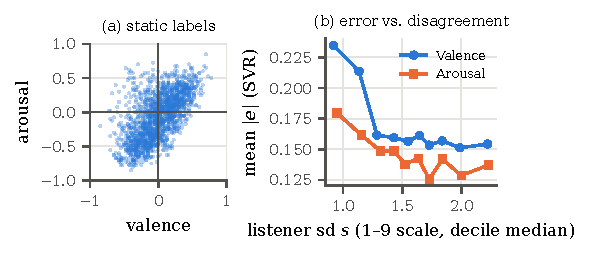
\includegraphics[width=\columnwidth]{fig_labels_disagreement}
\caption{(a) Static labels of the 1{,}744 clips after the correction of
Sec.~\ref{sec:res-swap}. (b) Mean absolute error of the SVR baseline per
decile of the listener standard deviation $s$: clips on which listeners
disagree more are predicted \emph{better}, not worse.}
\label{fig:labels}
\end{figure}

%======================================================================
\section{Design Decisions and Justification}
\label{sec:design}
%======================================================================
Table~\ref{tab:deviations} lists every change to the approved proposal and
its trigger. The main decisions are explained below.

% DRAFT deviation table (Efe): changes since the approved proposal, each with
% its reason. Needs \usepackage{booktabs,tabularx} in the preamble.
\begin{table*}[t]
\centering
\caption{Deviations from the approved proposal and their justification.}
\label{tab:deviations}
\footnotesize
\begin{tabularx}{\textwidth}{@{}p{2.6cm}XXp{2.2cm}@{}}
\toprule
\textbf{Aspect} & \textbf{Proposal} & \textbf{Now, and why} & \textbf{Trigger} \\
\midrule
Meaning of $\sigma$ &
$\sigma$ predicted by the NLL head expected to track listener disagreement (H2). &
$\sigma$ is defined as the predicted error of the model on the \emph{mean} rating
(model error plus averaging noise $\approx s^2/n$), not the spread of individual
listeners. $\rho(\sigma,s)$ is kept only as a descriptive analysis. H2 is split
into H2a (calibration, $\sigma$ vs.\ actual error), H2b (how measurable $s$ is)
and H2c (a head trained on individual ratings, after the report). &
Instructor feedback; Watcharasupat \emph{et al.}~\cite{watcharasupat2025} \\
Individual ratings &
Not considered. &
The data audit found per-rater static ratings (10--20 raters per clip, 187 raters),
which enables reliability ceilings now and explicit modelling of the rating
distribution (H2c) later. &
Instructor feedback; data audit \\
Split protocol &
One artist-disjoint 70/15/15 split, three seeds, bootstrap over test songs. &
Artist-grouped, quadrant-stratified 10-fold CV; fold $k{+}1$ is validation.
Every clip is tested exactly once, so uncertainty analyses use all 1{,}744
out-of-fold predictions instead of $\approx$262, and models are compared by
paired per-fold differences. &
Small dataset; \cite{bouthillier2021} \\
Success thresholds &
Fixed $R^2$ targets (e.g.\ C1: $R^2_V\geq0.30$, $R^2_A\geq0.60$; C2: $R^2_V\geq0.45$, $R^2_A\geq0.68$). &
C1 becomes a sanity check reported with its spread, not a pass/fail gate. The
primary H1 criterion is relative: the pretrained encoder must beat openSMILE
\emph{with the same head} on both dimensions. &
Instructor feedback (thresholds optimistic under artist-disjoint CV) \\
Same-head comparison &
SVR on openSMILE vs.\ MLP on MERT. &
Ridge and MLP heads are trained on both openSMILE and MERT so that the
representation effect is not confounded with the head; SVR is reported as an
additional baseline. &
Methodological \\
openSMILE excerpt &
DEAM features used as supplied. &
For the 744 clips of 2013 the supplied feature files cover the \emph{full song}
(up to 585\,s) while audio and ratings cover a 45\,s excerpt. Features are now
cropped to the excerpt using the segment start in the 2013 metadata (offsets
verified against the audio energy). &
Found during baseline work \\
2013 static labels &
Labels used as supplied. &
For the 744 clips of 2013 the static valence and arousal columns are swapped
relative to the dynamic annotations ($r\approx0.95$ crossed vs.\ $\approx0.57$
matched; 2014 is consistent) and to loudness. They are swapped back. &
Found during baseline work \\
2015 full songs &
Secondary out-of-distribution test set (58 songs). &
Dropped: different annotation protocol and only 5 raters per song. &
Scope \\
Scope of the report &
PANNs, fine-tuning and ensembles in weeks 3--5. &
PANNs, random-init MERT (null model), layer probe and LP-FT moved after the
report, following the instructor's ordering of priorities. &
Instructor feedback \\
\bottomrule
\end{tabularx}
\end{table*}


\subsection{What $\sigma$ represents}
\label{sec:sigma}
The instructor pointed out that a variance trained by NLL against the
\emph{mean} rating is not the variance between listeners. We adopt this as a
definition. Let $\bar y_i$ be the mean of $n_i$ ratings with listener standard
deviation $s_i$, and $f(x_i)$ the model's mean prediction. Then
\begin{equation}
\mathbb{E}\big[(\bar y_i - f(x_i))^2\big] =
\underbrace{(\mu_i - f(x_i))^2}_{\text{model error}} +
\underbrace{s_i^2/n_i}_{\text{averaging noise}},
\label{eq:sigma}
\end{equation}
where $\mu_i$ is the population mean rating. A well-trained $\sigma_i^2$
estimates this sum. It contains listener disagreement only through
$s_i^2/n_i$, which is divided by $n_i\approx10$, and it excludes epistemic
uncertainty, which we estimate separately with a seed ensemble. Consequently
we evaluate $\sigma$ in two clearly separated ways: (i) as a predictive
uncertainty, through calibration against $\bar y$ and its rank correlation
with the actual error $|e|$; (ii) descriptively, through its relation to $s$,
which we neither expect nor claim to be strong. The per-rater ratings found
by the audit allow the explicit modelling of the rating distribution that the
instructor suggested; this is planned as hypothesis H2c (a head trained on
individual ratings, giving $\sigma_{\text{listener}}$ to be compared with
$\sigma_{\text{mean}}$).

\subsection{Hypotheses after the feedback}
\begin{itemize}
\item \textbf{H1} (primary): with the same head, frozen MERT beats openSMILE on
both dimensions; MERT beats PANNs (secondary, after the report).
\item \textbf{H2a}: the heteroscedastic $\sigma$ is calibrated, ranks clips by
their actual error, and beats a constant $\sigma$.
\item \textbf{H2b}: how measurable is the clip-level disagreement $s$, and
does a frozen representation explain it beyond the mean rating?
\item \textbf{H2c}: a head trained on individual ratings measures something
different from a head trained on mean ratings.
\end{itemize}
The fixed numerical thresholds of the proposal are replaced by relative
criteria, as the instructor noted that they are optimistic for a small
dataset under an artist-disjoint protocol. The openSMILE result is a sanity
check reported with its spread (C1), and H1 is decided by paired per-fold
comparisons of the same head on two representations (C2).

\subsection{Evaluation protocol}
\textbf{Split.} We use artist-grouped, quadrant-stratified 10-fold
cross-validation (\texttt{StratifiedGroupKFold}, seed 415, groups = normalised
artist name, strata = valence--arousal quadrant). For test fold $k$, fold
$(k{+}1)\bmod 10$ is the validation set and the other eight folds train the
model ($\approx$80/10/10). All hyperparameters are chosen on validation only.
Compared to a single 70/15/15 split, every clip is tested exactly once, so the
uncertainty analyses use all 1{,}744 out-of-fold predictions instead of about
262, and models are compared fold by fold. Artist grouping prevents a model
from recognising an artist's timbre or production in the test set; a random
10-fold split is run for the baseline to measure this effect.

\textbf{Metrics.} For each dimension separately we report $\R$ (against the
test fold's mean), RMSE on the rescaled and on the 1--9 scale, the concordance
correlation coefficient
\begin{equation}
\mathrm{CCC} = \frac{2\rho\, s_y s_{\hat y}}{s_y^2 + s_{\hat y}^2 + (\bar y - \bar{\hat y})^2},
\end{equation}
which, unlike Pearson's $r$, also penalises bias and scale errors, and $r$.
For models with $\sigma$ we report the plain Gaussian NLL, the prediction
interval coverage probability at 68\,\% and 95\,\% (PICP), and Spearman
$\rho(\sigma, |e|)$. Models are compared through paired per-fold differences
(paired $t$-test and Wilcoxon signed-rank test). All metrics come from one
shared script that reads prediction files in a common format, so model code
never computes its own reported numbers.

\subsection{Representations and heads}
\textbf{openSMILE.} DEAM supplies 260 low-level descriptors per 500\,ms frame.
We summarise each by its mean and standard deviation over the 45\,s excerpt
(520 dimensions), standardised with training-fold statistics.

\textbf{MERT-v1-95M.} Audio is resampled to 24\,kHz and cut into nine 5\,s
windows; all 13 hidden layers ($13\times768$) are extracted in one pass and
cached, and the layer is selected on validation data. Pooling over windows
happens in the model code.

\textbf{Heads.} Ridge regression is the primary head for the same-head
comparison, because it has one hyperparameter and its result depends almost
only on the representation. An RBF-SVR is the classical MER
baseline~\cite{yang2008}, and a one-hidden-layer MLP (512 units) is the
nonlinear head shared with the heteroscedastic model.

\subsection{Numerical stability of the variance head}
\label{sec:stability}
The feedback asked us to guard against excessively small or large variances.
The heteroscedastic MLP outputs $(\mu, \sigma)$ per dimension with the
following safeguards:
\begin{itemize}
\item \textbf{Soft bounds:} $\sigma = \sigma_{\min} + (\sigma_{\max}-\sigma_{\min})\,\mathrm{sigmoid}(z)$,
instead of a hard clamp that would zero the gradient. $\sigma_{\min}=0.01$ is
below the averaging noise $s/\sqrt n\approx0.12$, and $\sigma_{\max}=2\,\mathrm{sd}(y_{\text{train}})$,
twice the error of a model that always predicts the training mean, beyond
which $\sigma$ carries no information.
\item \textbf{Warm-up:} $\mu$ is first trained with MSE only, then the loss
switches to $\beta$-NLL~\cite{seitzer2022} with $\beta=0.5$ (primary) and
$\beta=0$ (plain NLL, comparison), so that the variance cannot down-weight
hard examples before the mean has been learned.
\item \textbf{Selection:} weight decay, and early stopping and model selection
on the \emph{plain} validation NLL and RMSE, never on the $\beta$-NLL loss
value~\cite{seitzer2022}.
\item \textbf{Monitoring:} per epoch, the 1st/5th/50th/95th/99th percentiles of
$\sigma$ and the share of $\sigma$ within 1\,\% of either bound; if more than
5\,\% of validation $\sigma$ sit at a bound, this is reported as a stability
problem.
\end{itemize}
The reference for H2a is a homoscedastic model with the same $\mu$ and one
constant $\sigma$ per fold and dimension, the RMSE of the validation residuals.

%======================================================================
\section{Experiments and Results}
\label{sec:results}
%======================================================================
\subsection{Data audit and split integrity}
\label{sec:res-audit}
A scripted audit checks the annotation files, metadata and media:
\begin{itemize}
\item 1{,}744 clips, no missing or out-of-range $\mu$ or $s$; every clip has
an audio file and an openSMILE file.
\item Per-rater static ratings exist for every clip (10--20 raters). For one
clip (ID 1968) the averaged arousal differed from the rater mean by 0.62 and
was replaced by the rater mean.
\item Every clip has an artist; 898 distinct artists after normalisation
(case, whitespace, ``feat.''), 1--23 songs per artist, 596 single-song
artists, and 67 artists that appear in both years under one key.
\end{itemize}

The fold file passes an integrity test: every clip appears exactly once and
no artist appears in two folds. Folds hold 134--215 clips (86--93 artists);
the largest deviation of a fold's quadrant share from the overall share is
0.104. Fold sizes are uneven because the stratification balances quadrant
shares, not sizes, and some artists have up to 23 songs; we therefore report
fold metrics as mean~$\pm$~SD rather than re-splitting.

\subsection{Defect 1: swapped labels in the 2013 batch}
\label{sec:res-swap}
A first baseline run gave an implausible pattern: on the 2013 clips arousal
reached only $\R=0.29$, against $0.69$ on 2014. We therefore compared the
static labels of each clip with the time average of its dynamic annotations
(Fig.~\ref{fig:swap}). In 2014, static valence matches dynamic valence
($r=0.91$) and static arousal matches dynamic arousal ($r=0.94$). In 2013 the
pattern is crossed: static valence matches dynamic \emph{arousal} ($r=0.96$),
and static arousal matches dynamic \emph{valence} ($r=0.95$). Loudness, a
well-known arousal cue, gives independent evidence: in 2014 the mean RMS
energy correlates more with arousal than with valence (Spearman 0.42 vs.\
0.32), whereas with the supplied 2013 labels the order is reversed (0.54 vs.\
0.32). The per-rater file shows the same swap. We found no mention of this in
the DEAM manual. We swap the two columns back for the 744 clips of 2013 and
use the corrected labels everywhere.

\begin{figure}[t]
\centering
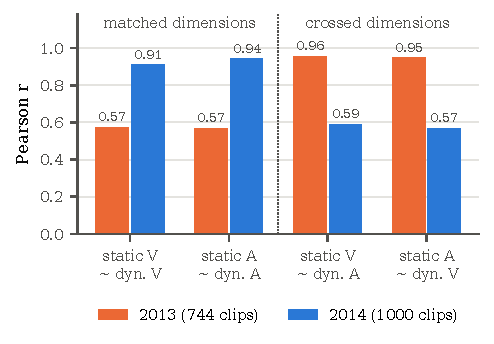
\includegraphics[width=\columnwidth]{fig_va_swap}
\caption{Correlation between the static labels and the time-averaged dynamic
annotations of the same clips. In 2014 the matching dimensions agree; in 2013
the crossed ones do, i.e.\ the static valence and arousal columns are swapped.}
\label{fig:swap}
\end{figure}

\subsection{Defect 2: full-song features for 2013}
For the 2013 clips the supplied openSMILE files cover the \emph{full song}
(up to 585\,s), whereas the audio file and the ratings cover a 45\,s excerpt
taken from a random point in the song. Averaging over the whole song mixes in
music the listeners never heard. We crop each file to the excerpt using the
segment start in the 2013 metadata (written as \textit{min.sec}). We verified
the offsets on 21 clips by locating the excerpt's RMS-energy curve, computed
from the mp3, inside the full-song openSMILE energy; all matched within one
frame (0.5\,s), with correlations up to 0.99.

Fig.~\ref{fig:fixes} shows the effect of both corrections on ridge. Cropping
raises both dimensions. The label fix moves the 2013 targets to the right dimension:
valence drops and arousal rises, because before the fix ``valence'' on 2013
was in fact the easier arousal target. With both fixes, the gap between the
batches closes (Table~\ref{tab:batch}).

\begin{figure}[t]
\centering
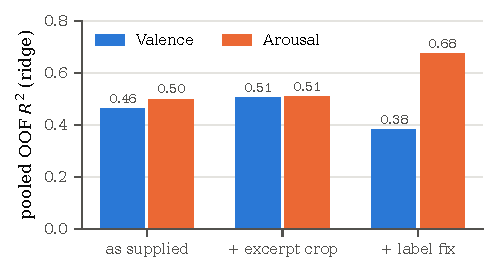
\includegraphics[width=\columnwidth]{fig_data_fixes}
\caption{Pooled out-of-fold $\R$ of the ridge baseline on artist-grouped
folds with the data as supplied, after cropping the 2013 features to the
annotated excerpt, and after also correcting the 2013 labels.}
\label{fig:fixes}
\end{figure}

\begin{table}[t]
\centering
\caption{SVR baseline by batch (pooled out-of-fold, cropped features).}
\label{tab:batch}
\footnotesize
\begin{tabular}{@{}lccccc@{}}
\toprule
 & & \multicolumn{2}{c}{supplied labels} & \multicolumn{2}{c}{corrected labels} \\
\cmidrule(lr){3-4}\cmidrule(l){5-6}
Batch & $n$ & $\R_V$ & $\R_A$ & $\R_V$ & $\R_A$ \\
\midrule
2013 & 744  & 0.608 & 0.292 & 0.367 & 0.645 \\
2014 & 1000 & 0.380 & 0.691 & 0.426 & 0.742 \\
\bottomrule
\end{tabular}
\end{table}

\subsection{openSMILE baseline}
Hyperparameters were selected per fold and dimension on validation RMSE:
ridge $\alpha\in10^{[-1,5]}$ (25 values; selected values mostly
$56$--$562$) and SVR $C\in\{0.1,0.3,1,3,10\}$,
$\gamma\in\{0.25,0.5,1,2\}/d$, $\epsilon\in\{0.02,0.05,0.1\}$. The model is
refit on the eight training folds and scored once on the test fold.
Table~\ref{tab:baseline} and Fig.~\ref{fig:folds} summarise the results; the
out-of-fold predictions are shown in Fig.~\ref{fig:scatter}.

\begin{table}[t]
\centering
\caption{openSMILE baselines, mean $\pm$ SD over 10 test folds.}
\label{tab:baseline}
\footnotesize
\setlength{\tabcolsep}{3pt}
\begin{tabular}{@{}llcccc@{}}
\toprule
Head & Dim & $R^2$ & RMSE & RMSE$_{1\text{--}9}$ & CCC \\
\midrule
Ridge & V & 0.372$\pm$0.079 & 0.216$\pm$0.017 & 0.865$\pm$0.068 & 0.563$\pm$0.070 \\
 & A & 0.671$\pm$0.061 & 0.189$\pm$0.017 & 0.756$\pm$0.068 & 0.806$\pm$0.041 \\
SVR & V & 0.379$\pm$0.075 & 0.215$\pm$0.012 & 0.859$\pm$0.049 & 0.565$\pm$0.063 \\
 & A & 0.693$\pm$0.045 & 0.183$\pm$0.013 & 0.731$\pm$0.051 & 0.822$\pm$0.029 \\
\midrule
Ridge (random split) & V & 0.395$\pm$0.046 & 0.215$\pm$0.008 & 0.859$\pm$0.034 & 0.579$\pm$0.042 \\
 & A & 0.677$\pm$0.036 & 0.189$\pm$0.010 & 0.757$\pm$0.042 & 0.810$\pm$0.020 \\
SVR (random split) & V & 0.414$\pm$0.047 & 0.211$\pm$0.009 & 0.845$\pm$0.035 & 0.599$\pm$0.033 \\
 & A & 0.698$\pm$0.031 & 0.183$\pm$0.009 & 0.732$\pm$0.034 & 0.823$\pm$0.020 \\
\bottomrule
\end{tabular}
\end{table}


\begin{figure}[t]
\centering
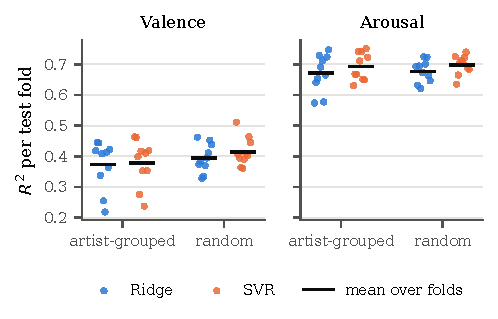
\includegraphics[width=\columnwidth]{fig_baseline_folds}
\caption{Per-fold test $\R$ of the openSMILE baselines on artist-grouped and
random folds. Each dot is one test fold.}
\label{fig:folds}
\end{figure}

\begin{figure}[t]
\centering
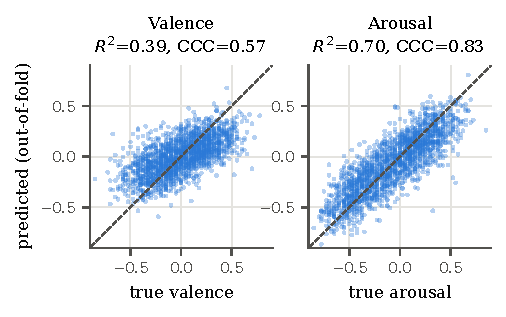
\includegraphics[width=\columnwidth]{fig_baseline_scatter}
\caption{Out-of-fold predictions of the SVR baseline (artist-grouped folds,
all 1{,}744 clips). Valence predictions shrink towards the centre.}
\label{fig:scatter}
\end{figure}

\textbf{Sanity check (C1).} The SVR reaches $\R_V=0.379$ and $\R_A=0.693$,
in line with the $0.32/0.64$ reported by Cheuk \emph{et al.}~\cite{cheuk2020}
and above the proposal thresholds of $0.30/0.60$. As in the literature,
arousal is much easier than valence; the CCC (0.57 vs.\ 0.82) and the scatter
show that valence predictions are also compressed towards the centre.

\textbf{Ridge vs.\ SVR.} SVR is better on arousal in 8 of 10 folds (mean
$\Delta\R=+0.022$, Wilcoxon $p=0.049$; $\Delta$CCC $=+0.015$, $p=0.020$). On
valence the two heads are indistinguishable (5/10 folds, $p=0.77$). The
nonlinear kernel thus helps little on this representation, which supports
ridge as the head for the same-head comparison with MERT.

\textbf{Artist effect.} Random folds are slightly easier: for SVR, $\R_V$
rises by 0.035 and $\R_A$ by only 0.005. Artist leakage therefore inflates
valence more than arousal, which supports the instructor's warning that
thresholds set from random-split results are optimistic under an
artist-disjoint protocol. Its size for pretrained embeddings, which may encode
artist identity more strongly, is an open question that we will test.

\textbf{Headroom.} The noise ceiling of the mean rating,
$1-\overline{s^2/n}/\mathrm{Var}(\mu)$, is $0.79$ (valence) and $0.85$
(arousal). Averaging noise alone accounts for about 35\,\% (valence) and
50\,\% (arousal) of the SVR's mean squared error, so there is substantial room
for a better representation, especially on valence.

\subsection{What the listener disagreement can and cannot tell us}
\label{sec:res-disagreement}
Before training a variance head we asked how informative the per-clip listener
standard deviation $s$ is. Using the per-rater ratings, we computed
split-half reliabilities (500 random 5/5 splits of each clip's raters,
Spearman--Brown corrected to 10 raters):
\begin{itemize}
\item The \emph{mean} rating is reliable: 0.79 (valence) and 0.85 (arousal).
\item The \emph{standard deviation} $s$ is not: 0.00 (valence) and 0.05
(arousal). After removing each rater's bias and scale with an additive
clip~+~rater model fitted out-of-sample, it rises only to 0.21 and 0.14.
\end{itemize}
With 10 raters, the clip-to-clip differences in $s$ are almost entirely
sampling noise. Any correlation with raw $s$ is therefore capped near
$\sqrt{0.05}\approx0.2$, and near $0.4$ for the rater-adjusted $s$. This
explains why earlier work found that models do not reproduce listener
disagreement~\cite{watcharasupat2025}.

The baseline errors make the second half of the argument. The Spearman
correlation between $|e|$ and $s$ is \emph{negative}: $-0.15$ for valence and
$-0.10$ for arousal ($p<10^{-4}$, Fig.~\ref{fig:labels}b). Clips near the
centre of the scale have more disagreement (Spearman $\rho(|\mu|,s)=-0.23$ and
$-0.30$; a mean near the end of a bounded scale forces a small spread), while
extreme clips are the hardest to predict, because regression shrinks towards
the centre. With the rater-adjusted $s$ the correlation vanishes ($0.00$ and
$-0.03$, n.s.). A $\sigma$ that tracks the model's own error, which is what
NLL training against the mean rating rewards (Eq.~\ref{eq:sigma}), can thus
not be expected to correlate positively with listener disagreement. This is
the empirical counterpart of the distinction drawn in the feedback, and it
fixes how we will interpret $\rho(\sigma, s)$: as a descriptive quantity,
reported with its ceiling and with partial correlations that control for
$\mu$ and $\hat\mu$.

\subsection{Homoscedastic reference}
The constant-$\sigma$ reference, with $\sigma$ equal to the validation RMSE,
is already calibrated on average: PICP$_{68}=0.67$--$0.68$ and
PICP$_{95}=0.94$--$0.95$ for both heads and dimensions, with test NLL
$-0.11$ (valence) and $-0.24$ (arousal) for ridge. By construction its
$\rho(\sigma,|e|)$ is zero. A heteroscedastic head must therefore improve on
NLL and on the ranking of errors, not merely reach nominal coverage, to
support H2a.

\subsection{Work in progress}
\textbf{MERT.} The extraction script (all 13 layers, nine 5\,s windows at
24\,kHz per clip, float16 cache) is implemented and was tested on a GPU; the
cache for all 1{,}744 clips had not been completed at the time of writing. MERT is unaffected by the
feature defect because it reads the 45\,s audio directly. Once the cache is
available, ridge and the MLP will be trained on it with the same folds and
compared fold by fold with Table~\ref{tab:baseline}.

\textbf{Heteroscedastic head.} A prototype with soft-bounded $\sigma$, an MSE
warm-up and NLL training with early stopping runs end-to-end on openSMILE
features. Its first results were obtained with the uncorrected 2013 labels and
an earlier split, so we do not report them; it will be rerun with the
corrected labels on the shared folds, with the stability logging of
Sec.~\ref{sec:stability}.

%======================================================================
\section{Summary and Next Steps}
\label{sec:conclusion}
%======================================================================
\textbf{Done.} Following the priorities in the feedback, we (i) audited the
annotations, artist identifiers and media and built an artist-grouped,
quadrant-stratified 10-fold protocol that passes its integrity test;
(ii) found and corrected two undocumented defects in the 2013 part of DEAM,
swapped static valence/arousal labels and full-song openSMILE features;
(iii) established the openSMILE baseline, SVR $\R=0.379/0.693$ and CCC
$=0.565/0.822$ on artist-disjoint folds, consistent with the literature;
(iv) quantified the artist effect (larger for valence); and (v) made precise
what a mean-trained $\sigma$ represents and showed that the per-clip listener
disagreement is nearly unmeasurable with 10 raters and negatively related to
model error. We also implemented the shared metric script, the prediction
format, the homoscedastic reference and the MERT extraction.

\textbf{Next steps.}
\begin{enumerate}
\item Finish the MERT cache; train ridge (layer chosen on validation) and the
MLP on MERT and on openSMILE; test H1 by paired per-fold comparisons, and
measure the artist effect for MERT.
\item Rerun the heteroscedastic head on the corrected labels ($\beta=0.5$ and
$0$); report calibration (PICP, reliability diagram, ENCE), $\rho(\sigma,|e|)$
against its simulated ceiling, NLL against the homoscedastic reference, and the
stability diagnostics; add a seed ensemble for the epistemic part.
\item Decompose $\sigma^2$ descriptively into averaging noise $s^2/n$,
ensemble variance and distance from the scale centre, to answer what the
predicted uncertainty represents.
\item After the basic pipeline: PANNs (H1, secondary), a randomly initialised
MERT as a null model for the disagreement probe (H2b), and a head trained on
individual ratings (H2c); fine-tuning (LP-FT) only if time permits.
\end{enumerate}

\bibliographystyle{IEEEtran}
\bibliography{refs}

\end{document}
